\section{Virtual Private Networks}

How to interconnect geographically distributed sites with the same privacy and guarantees as a private network on top of a shared infrastructure? High-level goals: support multiple customers, provide QoS guarantees, easy to use and manage for customer and provider.

\subsection{User-Managed VPN}

In a customer-managed VPN, provider is agnostic and simply provides dedicated physical connections (solution 1) or IP connectivity (solution 2).

\paragraph{Solution 1: Leased-Line}
A dedicated (private) full-duplex symmetrical connection between two geographically distant sites according to a commercial contract (e.g. provided by Swisscom). QoS guarantees easy since connection is dedicated and does not carry third-party communications. Either organized as a full mesh connecting all sites pairwise (redundancy) or as a hub-and-spoke where all sites are reachable but not specifically direct neighbors (cheaper).

Quality of connections is typically very good but it can be very expensive since you need many LLs (at least one per site). With $n$ sites and for a full mesh, one needs $\frac{n(n-1)}{2}$ LLs and $n$ interfaces on each router. Also, LL-based VPNs are not flexible since adding an LL can take months and adding / removing a site is a logistic nightmare.

\paragraph{Solution 2: IP-Based}
On each site, customer contracts simple IP connectivity with one or more providers (different IP subnets!). The customer then creates IP tunnels between its sites. The provider only needs to know the public IP addresses (11.0.0.0/8 in the example).

\textbf{IP Tunnel:} forwarding traffic across network that wouldn't normally support it (no existing native routing path to each other. Encapsulate traffic s.t. it carries a different header (= native) which the carrier network can process. There exist other tunneling protocols, plus IPsec also encrypts the original packet.

\begin{figure}[h]
	\centering
	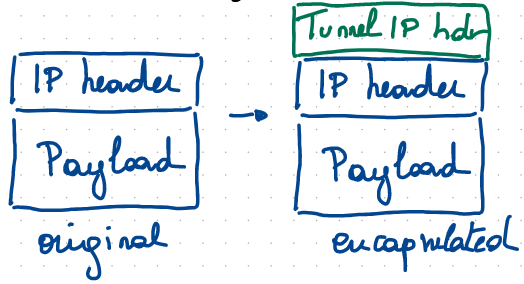
\includegraphics[scale=0.5]{images/3-tunnel.PNG}
	\caption{Additional IP header for tunneling (IP in IP) with source and destination addresses of the gateway routers.}
	\label{fig:tunnel}
\end{figure}

\begin{figure}[h]
	\centering
	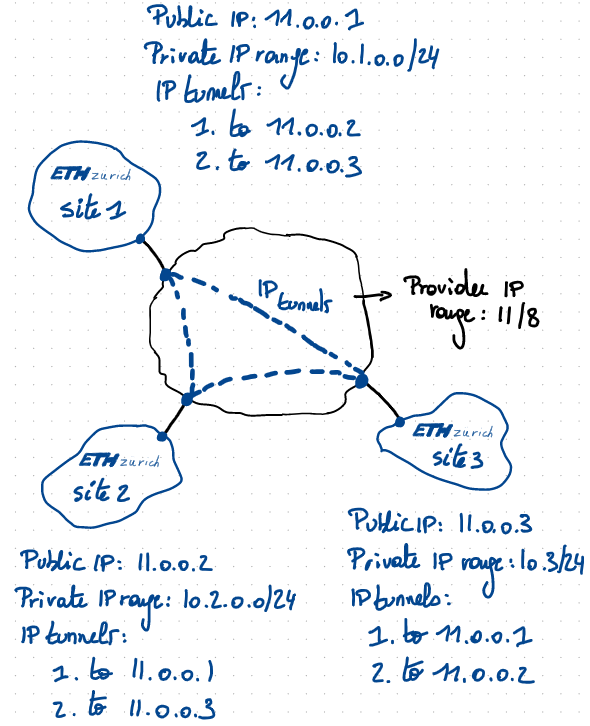
\includegraphics[scale=0.7]{images/3-ipexample.PNG}
	\caption{IP-based VPN infrastructure. Gateway routers native to transit network determine the tunnel to use and encapsulate outgoing packets accordingly.}
	\label{fig:ipexample}
\end{figure}

\textbf{Generic Routing Encapsulation (GRE):} can encapsulate many different protocols inside virtual point-to-point / to-multipoint links over IP (encapsulated packet has both an IP and a GRE header). GRE enables to give an insight into which protocol is encapsulated. See Figure \ref{fig:gre}.

\begin{figure}[h]
	\centering
	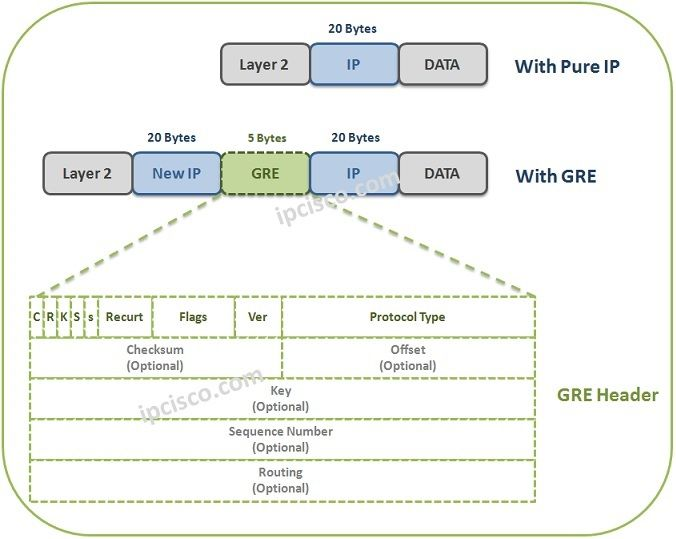
\includegraphics[scale=0.5]{images/3-gre.jpg}
	\caption{GRE header specification (note: Protocol Type indicating encapsulated protocol = EtherType).}
	\label{fig:gre}
\end{figure}

\textbf{Pros and Cons:} Much cheaper since each router (in each site) only requires one interface to connect to all others (or two for redundancy) since traffic is multiplexed. Again, total number of tunnels can be high (see full mesh connections). Adding a new site requires router config modification at all sites (if full mesh). Few guarantees are provided since provider is unaware that it is dealing with VPN traffic - only best-effort. VPN security depends on tunneling mechanism (weak for GRE, good for IPsec).


\subsection{Provider-Managed VPN}

The customer is agnostic to the service and it looks like the different sites are directly connected together through the provider. See Figure \ref{fig:provider} for an example architecture.

\begin{figure}[h]
	\centering
	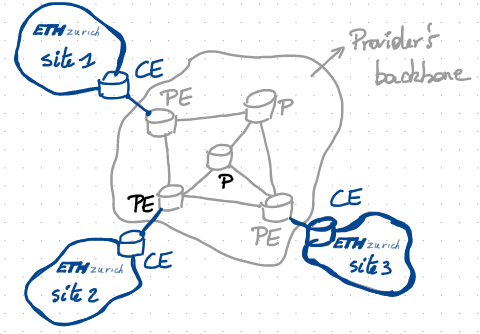
\includegraphics[scale=0.7]{images/3-provider.PNG}
	\caption{Architecture of a provider-managed VPN with CE, PE and P routers.}
	\label{fig:provider}
\end{figure}

\paragraph{Customer Edge (CE)}
Router sending IP packets through ISP backbone to reach other sites of the VPN. Always connected to a PE and does not now any details of ISP backbone.

CE routers only need one routing table containing routers of their own VPN (e.g. reach own site via local routing, reach different site via specific PE).

\paragraph{Provider Edge (PE)}
Maintains per-VPN config and ensures that packets sent by a site are delivered to PE attached to destination site.

In addition to the default routing table (backbone routes) they also maintain a dedicated routing table for each VPN a PE router is attached to - known as a VPN Routing and Forwarding table (VRF). Two packets from different VPNs with the same destination can map to different routes (next-hops) in their respective VRF on a PE router. See Figure \ref{fig:vrf} for an example.

\begin{figure}[h]
	\centering
	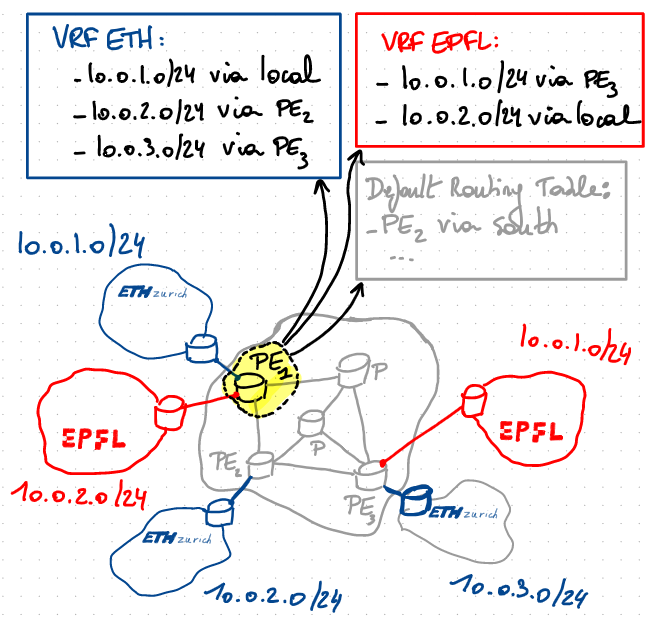
\includegraphics[scale=0.6]{images/3-vrf.PNG}
	\caption{Examples of VRFs for two VPNs.}
	\label{fig:vrf}
\end{figure}

%TODO: how are these packets marked / distinguished?

\paragraph{Provider (P)}
Routers withing ISP backbone. Unaware of VPN service.

P routers only need one routing table containing the routes of the backbone (how to reach P and PE routers).

%TODO hands-on example lec 8

\subsubsection{Routing}

%TODO difficult, check again, draw this? lec 8, print notes, examples

\paragraph{Distributing Routing Information}
First, each CE must advertise its local routes to its connected PEs. PEs in turn advertise the remote VPN routes to the CE (via static routes / configuration, eBGP, RiP, etc.).

Then, each PE must receive per-VPN routes reachable through local CE routers / remote PE routers and internal ISP routes to reach other PE routers (infrastructure routes, often going through a P router - plain OSPF).

Lastly, PE routers only advertise / receive internal routes. They don't know anything about VPN routes.

\begin{figure}[h]
	\centering
	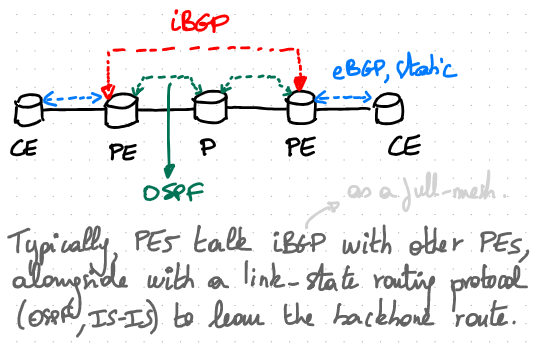
\includegraphics[scale=0.6]{images/3-routing.PNG}
	\caption{First and second step of distributing routing information.}
	\label{fig:routing}
\end{figure}

\paragraph{Dealing With Conflicting Info}
Different VPNs can use the same internal address space (e.g. ETHZ and EPFL both use 10.0.0.0/8) - same destination IP can map to different sites belonging to different VPN. Also, we want the CEs to only learn routes pertaining to their own VPN.

Concatenate a unique value to the IP address corresponding to the addressed VPN (8-byte Route Distinguisher, RD = 96-bit total address) and exchange that with Multiprotocol-BGP (MP-BGP) to solve the first problem.

Restrict the distribution of VPN-IPv4 routes using labels by assigning a unique label (= Route Target) to each VPN and have the PE router attach the tag to the BGP route before propagating it on iBGP. A PE router then only inspects routes associated with a given tag where they have a connected CE router.

Typically, both these labels are the same (RD and RT).


\subsubsection{Forwarding}

CE routers send pure IP packets, PE router encapsulates these with two MPLS labels (outer label identifying next-hop PE and inner label identifying VRF to use in remote PE).